% vim: set spelllang=fr:

\setchapterpreamble[ur][.6\textwidth]{%
  \dictum[Bill Watterson, \textit{Calvin et Hobbes}]{%
    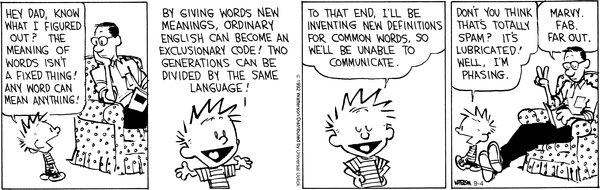
\includegraphics[width=0.6\textwidth]{fig/calvin_meaning.png}}}

\chapter{Annotation en rôle sémantique en domaine spécifique}
\label{ch:domainsrl}

% TODO  ?
% Evaluating our approach on domain-specific corpora such as the Kicktionary
% \citep{schmidt2009kicktionary}, the Robocup dataset \citep{chen2008learning} or
% the Situated Language dataset \citep{bordes2010towards} and compare our method
% with existing domain-specific semantic role labeling work
% \citep{wyner2010lexical,hadouche2011annotation,goldwasser2013leveraging}.


Là où le précédent chapitre présentait sur l'annotation en rôles sémantiques
fondée sur la connaissance, celui-là se concentre sur l'annotation en domaines
spécifiques.

La définition du terme 'domaine' reste assez vague dans le sens où il est
difficile de proposer une catégorisation de la connaissance en un ensemble de
domaines qui soit à la fois cohérente et efficace pour le Traitement Automatique
des Langues. Il est aussi difficile de séparer clairement le «~domaine
général~» des domaines spécifiques.

% TODO wordnet domains issues ma2012rethinking

Néanmoins, c'est un phénomène qui existe et qui est à considérer : les modèles
entraînés sur un corpus d'un domaine spécifique (la finance par exemple)
généraliseront mal à d'autres domaines (le football) par exemple. % proof

À l'heure où les algorithmes supervisés obtiennent d'excellentes performances
sur un certain nombre de tâche, l'adaptation au domaine est un défi majeur du
Traitement Automatique des Langues.

Il est important aussi de différencier le genre et le domaine d'un texte. Le
corpus du Wall Street Journal traite du domaine de la finance dans un genre
journalistique. D'autres genres existent, par exemple les genre littéraires que
sont la fiction, la poésie, le théâtre, etc. Néanmoins, ces distinctions ne
nous concernent pas ici, et l'objectif affiché est de traiter aussi bien un
roman qu'une encyclopédie qu'un email bien écrit qu'un article de journal.
C'est une simplification mais les difficultés que nous rencontrons avec les
corpus utilisés dépendent plutôt du domaine que du genre. En effet, dans deux
domaines différents plus que dans deux genres différents, les changements vont
résider dans les verbes utilisés, leur sens et la façon de les utiliser. C'est
ce que nous souhaitons prendre en compte ici.

\section{Corpus considérés}

Afin de s'assurer que notre travail reste valide en changeant de domaine, nous
considérons ici trois corpus présents dans des domaines différents :

\begin{itemize}
    \item le Kicktionary rassemblant des dépêches de l'UEFA dans le domaine du football,
    \item DicoInfo~: corpus Informatique/Internet de l'OLST,
    \item et DicoEnviro~: le corpus Réchauffement climatique de l'OLST
\end{itemize}

Les points communs majeurs de ces trois corpus sont :
\begin{enumerate}
    \item de s'inspirer librement de la théorie des Frame Semantics telle qu'elle est considérée dans FrameNet,
    \item d'être disponible à la fois en anglais et en français,
    \item d'être basés sur l'annotation dans un corpus d'un certain nombre de prédicats (ce n'est pas une annotation dite "full-text")
\end{enumerate}

Ce dernier point est plutôt un inconvénient : la manière la plus réaliste de
considérer un corpus d'entraînement est de réaliser une annotation dite
\textit{full-text} en annotant tous les prédicats rencontrés dans un texte
donné. Cependant, les contextes choisis dans DicoInfo et DicoEnviro l'ont été
sur des critères de diversité syntaxique. \citep{lhomme2012adding} Le postulat
que nous faisons dans ce travail est que notre méthode n'est pas affectée par
ce problème comme le serait un modèle statistique appris sur ces mêmes
contextes étant donné que la probabilité des différentes possibilités n'est pas
prise en compte.

\section{Enrichissement de VerbNet}

Malgré leur similarité, ces corpus posent des problèmes différents vis-à-vis de
leur annotation avec VerbNet, tous liés au fait de ne pas être dans le "domaine
général". Nous avons considéré comme problème les manquements dans VerbNet qui
empêchent de prendre en compte les phrases considérées, indépendamment de
l'algorithme. Ainsi, pour que VerbNet puisse prendre en compte une instance, il
faut :

\begin{itemize}
    \item que le sens du verbe considéré soit présent dans VerbNet,
    \item que la construction en question soit présente dans VerbNet,
    \item et que les rôles sémantiques associés à chaque syntagme soient correct.
\end{itemize}

Il y a différentes façons de ne pas respecter ces contraintes :

\begin{itemize}
    \item Le verbe n'existe pas du tout dans VerbNet
    \item Le sens du verbe utilisé n'est pas représenté dans VerbNet alors que c'est un sens du domaine général
    \item Le sens du verbe utilisé n'est pas représenté dans VerbNet alors que c'est un sens spécifique à ce domaine
    \item La construction utilisée n'est pas présente dans VerbNet
    \item La construction utilisée est incorrecte dans VerbNet
\end{itemize}

Suivant les corpus considérés, les proportions d'erreurs seront différentes.
Nous avons demandé à deux annotateurs d'évaluer, pour vingt phrases par
domaine, quelle était l'erreur. L'accord inter-annotateur permet de valider la
distinction domaine spécifique/domaine général malgré l'impossibilité de la
définir précisément. % TODO lefaire

C'est pour cette raison que l'enrichissement de VerbNet se fait de deux
manières : certains verbes et constructions sont ajoutés comme faisant partie
du domaine général, alors que d'autres sont étiquetés avec le domaine
spécifique correspondant. L'idée est d'éviter que des connaissances de domaines
spécifiques viennent réduire la qualité de la ressource tout en s'assurant que
la couverture de VerbNet pour le domaine général continue de s'améliorer.

\subsection{Détection semi-automatique d'erreurs}

D'une part, pour minimiser le travail manuel, il est important d'automatiser au
maximum l'enrichissement de la ressource. D'autre part, l'intérêt de VerbNet
réside notamment dans sa capacité à factoriser efficacement ces informations
sur l'interface syntaxico-sémantique d'un verbe donné, et il est donc possible
et utile de valider manuellement chacun des changements apportés.

Le principe suivi est donc d'essayer de détecter les manquements de VerbNet de
manière automatique avant de proposer à un utilisateur expert de réaliser des
changements en ayant un maximum d'informations pertinentes à portée de main.

Les différentes erreurs détectées sont :
\begin{itemize}
    \item l'absence de lemmes dans la ressource
    \item l'absence d'un sens correct dans la ressource
    \item l'absence de constructions correctes dans la ressource
    \item l'absence de mapping de role correct dans la ressource
\end{itemize}

Nous avons d'abord commencé par détecter l'absence de constructions correctes,
ce qui a permis ensuite de détecter une absence de sens en comparant les
constructions observées avec les constructions présentes. Enfin, cela a permis
de faire des propositions quant à la position d'un nouveau lexème dans la
ressource.

\section{Méthode d'évaluation}

Les trois corpus considérés ont été annotés en rôles sémantiques dans les deux
langues qui nous intéressent ici~: l'anglais et le français. Il nous suffit
donc d'utiliser un mapping entre les rôles considérés par ces ressources et les
rôles VerbNet avant d'évaluer la performance de l'algorithme basé sur la
connaissance d'annotation en rôles sémantiques présenté au
chapitre~\ref{ch:srl}.

Dans le cas de DicoInfo et DicoEnviro, les noms des rôles sont proches des noms
de rôles employée dans VerbNet et LIRICS \citep{bonial2011hierarchical} (Agent,
Patient, Destination, Instrument...). Cependant, même si les noms sont les
mêmes, la définition de ces rôles est spécifique à DicoInfo et DicoEnviro.
En pratique :

\begin{itemize}
    \item DicoInfo et DicoEnviro ne distinguent pas Theme de Patient mais
    n'utilise que Patient ce qui rend l'annotation plus facile.\footnote{La
    distinction entre Theme et Patient est difficile à établir. Dans \textit{Le
    chaton a léché mes doigts}, est-ce que mes doigts ont changé d'état ? Si oui,
    ils devraient être Patient, et sinon, Theme.\citep[p.~5]{palmer2010semantic}}
    \item Pour un certain nombre de lexies, la perspective du domaine implique
    souvent des rôles différents (TODO exemple Patient vs. Result) % TODO clair
\end{itemize}

C'est pour ces raisons que nous avons créé manuellement un mapping entre
VerbNet et les corpus considérés (DicoInfo et DicoEnviro). Ce mapping est
utilisé uniquement à des fins d'évaluation, et l'effort nécessaire pour le
créer n'est donc pas à prendre en compte pour calculer l'effort global
nécessaire pour notre approche. Prenons deux phrases d'exemple pour illustrer
le mapping. Voici deux phrases présentes dans DicoInfo et DicoEnviro :

\begin{itemize}
    \item In the interest of fair competition you should ALLOCATE the same amount of memory to both engines.
    \item Techniques and tools exist to MEASURE carbon stocks in project areas relatively precisely depending on the carbon pool.
\end{itemize}

Dans la première phrase, le sens du verbe \textit{allocate} est très précis et
très spécifique au domaine de l'informatique. Pourtant, il se comporte
syntaxiquement de la même manière que le sens plus général considéré par
WordNet et OntoNotes: \textit{distribute or se aside according to plan}. Par
conséquent, un mapping manuel a été réalisé de la lexie allocate.1 (qui
correspond à la phrase ci-dessus) vers la classe Verbnet
\textit{future\_having-13.3}. Enfin, les actants définis par DicoInfo (qui
correspondent aux roles \textit{Core} de FrameNet et aux rôles de VerbNet) ont
étés mis en correspondance avec les rôles de VerbNet :

\begin{itemize}
    \item Patient devient Theme
    \item Recipient devient Goal
    \item Agent reste Agent
\end{itemize}

Une fois que ce mapping est réalisé, la tâche de notre algorithme d'annotation
en rôles sémantiques devient de détecter que la classe future\_having-13.3 est
utilisée ici, que 'You' est Agent, que 'the same amount of memory' est Theme,
et que 'to both engines' est Goal. La démarche est la même pour la seconde
phrase, où il s'agit d'identifier que \textit{Techniques and tools} est Agent,
et que \textit{carbon stocks} est Theme.

\section{Résultats}
